% !TeX spellcheck = ru_RU
% !TEX root = vkr.tex

\section{Описание решения}
\label{sec:solution}
\subsection{Иерархия классов}

Общая иерархия классов, связанных с условными зависимостями включения, представлена на рис.~\ref{fig:cind_hierarchy}. Базовый класс \texttt{Algorithm} определяет единый жизненный цикл всех алгоритмов в Desbordante: загрузка данных (\texttt{LoadData}), конфигурация параметров (\texttt{SetOption}) и выполнение (\texttt{Execute}). Каждый алгоритм реализует три чисто виртуальных метода: \texttt{LoadDataInternal}, \texttt{ExecuteInternal} и \texttt{ResetState}.

Класс \texttt{CindAlgorithm} реализует полный пайплайн поиска CIND. Внутри он создаёт экземпляр алгоритма \texttt{Spider} для обнаружения приближённых зависимостей включения, а затем передаёт найденные AIND одному из майнеров условий~--- \texttt{Cinderella} или \texttt{PliCind}, выбираемому через параметр \texttt{AlgoType}. Оба майнера наследуются от абстрактного класса \texttt{CindMiner}, который определяет интерфейс для поиска условий.

Класс \texttt{CINDVerifier}, реализованный в рамках данной работы, также наследуется от \texttt{Algorithm} и предоставляет функциональность верификации~--- проверки того, выполняется ли заданная CIND на конкретных данных. В отличие от \texttt{CindAlgorithm}, верификатор не выполняет поиск, а проверяет одну конкретную зависимость с заданным условием.

\begin{figure}[H]
\centering
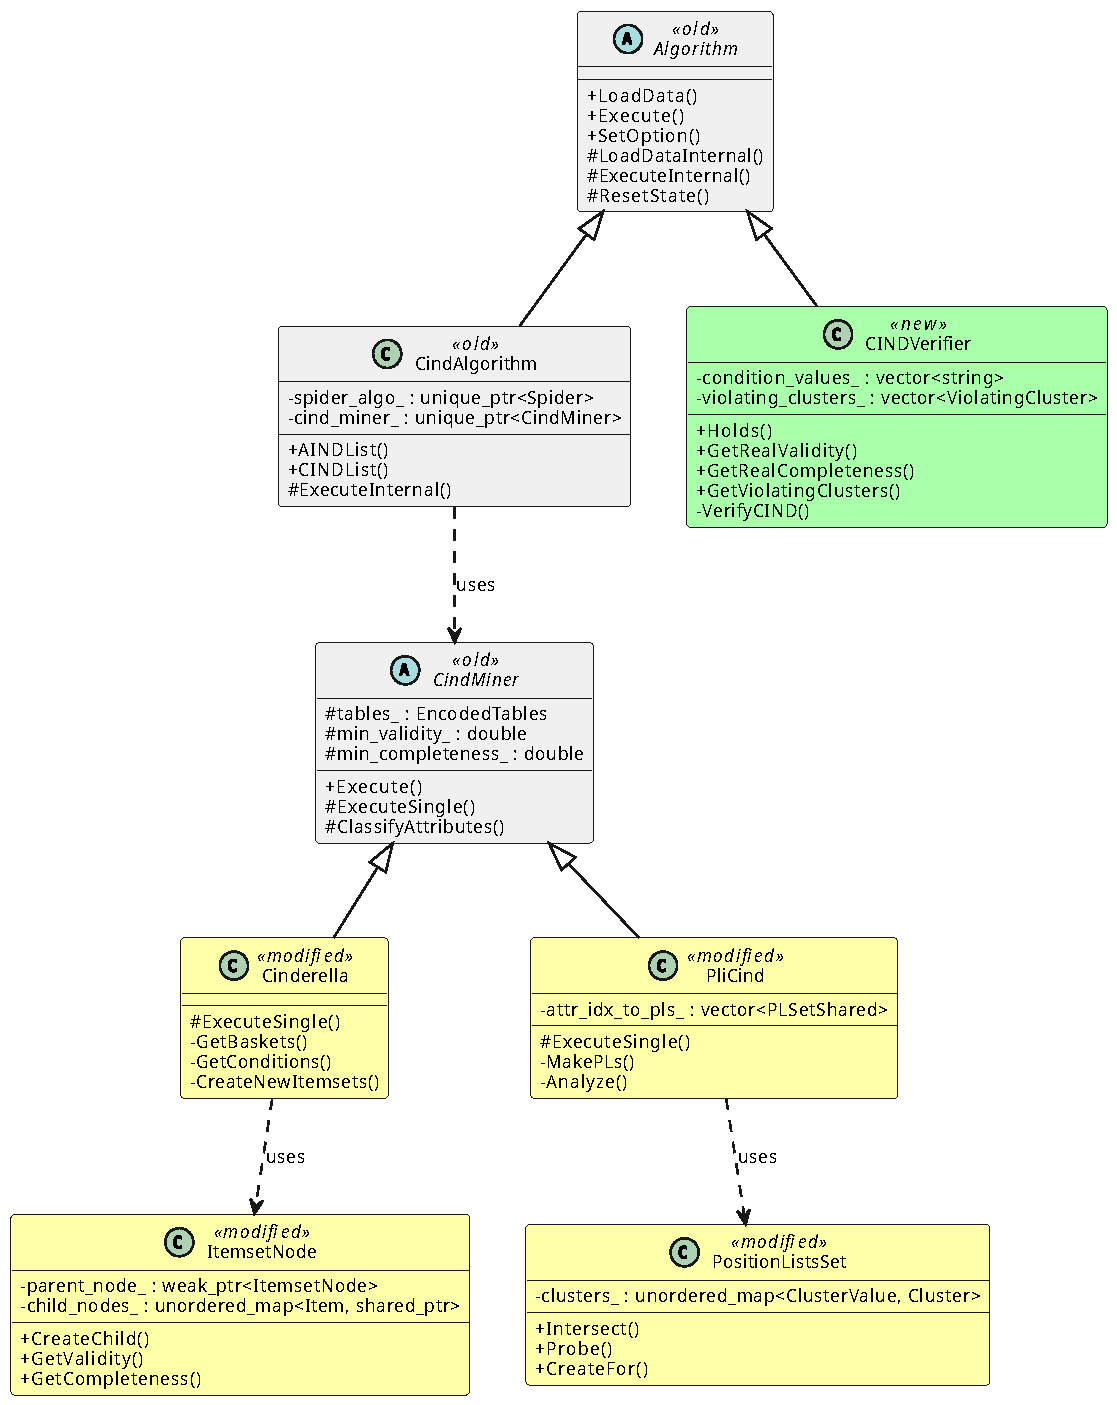
\includegraphics[width=\textwidth]{cind_uml.png}
\caption{UML-диаграмма классов для поиска и верификации CIND. Сплошные стрелки~--- наследование, пунктирные~--- использование.}
\label{fig:cind_hierarchy}
\end{figure}

\noindent Обозначения цветов на диаграмме:
\begin{itemize}
    \item \textbf{Серый}~--- классы, не затронутые в данной работе (\texttt{Algorithm}, \texttt{CindAlgorithm}, \texttt{CindMiner});
    \item \textbf{Жёлтый}~--- классы, в которых проведены оптимизации (\texttt{Cinderella}, \texttt{PliCind}, \texttt{ItemsetNode}, \texttt{PositionListsSet});
    \item \textbf{Зелёный}~--- классы, реализованные в данной работе (\texttt{CINDVerifier}).
\end{itemize}

\subsection{Алгоритм верификации}

Класс \texttt{CINDVerifier} принимает на вход две таблицы, индексы атрибутов включения для каждой из них, а также набор значений условия. Поддерживаются оба типа условий: строковые (\texttt{row}) и групповые (\texttt{group}), задаваемые через параметр \texttt{condition\_type}.

Алгоритм верификации работает в два этапа.

\textbf{Этап~1. Построение множества включённых значений.} Из правой таблицы $I_2$ извлекаются все уникальные комбинации значений атрибутов включения $Y$ и помещаются в хеш-множество. Это позволяет за время $O(1)$ проверять, является ли конкретный кортеж из $I_1$ включённым.

\textbf{Этап~2. Проверка кортежей левой таблицы.} Кортежи из $I_1$ группируются по значениям атрибутов включения $X$. Для каждой группы определяется:
\begin{enumerate}
    \item является ли группа включённой (присутствует ли значение $x$ в хеш-множестве из этапа~1);
    \item удовлетворяют ли кортежи группы заданному условию.
\end{enumerate}

Если все значения условия являются подстановочными символами, верификатор использует упрощённый путь: проверяется только включённость каждой группы без фильтрации по условию. В противном случае для каждого кортежа выполняется сопоставление с условием: закодированное значение каждого атрибута условия сравнивается с ожидаемым значением, причём подстановочные символы пропускаются.

Группы, содержащие кортежи, удовлетворяющие условию, но не являющиеся включёнными, фиксируются как нарушающие. Для каждой такой группы создаётся объект \texttt{ViolatingCluster} с индексами всех строк группы и индексами строк-нарушителей.

По завершении обхода вычисляются метрики:
\[
\operatorname{validity} = \frac{\text{included\_support}}{\text{supporting\_baskets}}, \qquad
\operatorname{completeness} = \frac{\text{included\_support}}{\text{included\_baskets\_total}},
\]
где \texttt{supporting\_baskets}~--- число групп (или строк), удовлетворяющих условию, \texttt{included\_support}~--- число таких групп, которые при этом являются включёнными, а \texttt{included\_baskets\_total}~--- общее число включённых групп.

\subsection{Оптимизация алгоритмов поиска условий}

Первоначальная реализация алгоритмов CINDERELLA и PLI-CIND, выполненная в рамках бакалаврской работы~\cite{abrosimov2025cinderella}, использовала структуры данных, не оптимальные с точки зрения производительности. В данной работе были проведены оптимизации обоих алгоритмов, направленные на снижение вычислительной сложности ключевых операций и повышение эффективности использования памяти.

Основные направления оптимизации можно разделить на три группы.
\begin{itemize}
    \item \textbf{Замена упорядоченных контейнеров на хеш-контейнеры.}\\ 
    Контейнеры с логарифмической сложностью операций, использовавшиеся для хранения множеств значений правой таблицы и индексов групп, были заменены на их неупорядоченные аналоги. Это позволило снизить сложность операций поиска и вставки с $O(\log n)$ до амортизированного $O(1)$, что существенно при обработке таблиц с большим числом уникальных значений.

    \item \textbf{Улучшение кэш-локальности и сокращение аллокаций.}\\
    Связные списки, применявшиеся для хранения информации о корзинах и позиций строк, были заменены на непрерывные массивы с предварительным резервированием памяти. Последовательное размещение данных обеспечивает более эффективное использование процессорного кэша и сокращает накладные расходы на динамическое выделение памяти.

    \item \textbf{Устранение избыточных вычислений.}\\
    Устранены повторные обращения к ассоциативным контейнерам, поэлементные копирования коллекций заменены на перемещения с использованием move-семантики, а линейный поиск по дочерним узлам дерева наборов элементов заменён на обращение по ключу через хеш-таблицу.
\end{itemize}

\subsection{Интеграция в Desbordante}

\subsubsection{Пользовательские параметры}

Верификатор \texttt{CINDVerifier} предоставляет следующие параметры, задаваемые через систему опций Desbordante:

\begin{itemize}
    \item \texttt{tables}~--- список входных таблиц (минимум две: левая и правая);
    \item \texttt{lhs\_indices}~--- индексы атрибутов включения в левой таблице;
    \item \texttt{rhs\_indices}~--- индексы атрибутов включения в правой таблице;
    \item \texttt{cind\_condition\_values}~--- список значений условия, выровненный по порядку атрибутов условия (подстановочный символ \texttt{"-"} или \texttt{"\_"} для произвольного значения);
    \item \texttt{condition\_type}~--- тип условия: \texttt{"row"} для строковых или \texttt{"group"} для групповых метрик.
\end{itemize}

Атрибуты условия определяются автоматически как все столбцы левой таблицы, не входящие в \texttt{lhs\_indices} (а при верификации в рамках одной таблицы~--- также не входящие в \texttt{rhs\_indices}).

\subsubsection{Python-биндинги}

Верификатор доступен из Python через модуль \texttt{cind\_veri\-fi\-ca\-tion} пакета \texttt{desbordante}. Биндинги реализованы с помощью библиотеки pybind11 и предоставляют следующий интерфейс:

\begin{itemize}
    \item \texttt{holds()}~--- возвращает \texttt{True}, если CIND выполняется с заданными порогами;
    \item \texttt{get\_real\_validity()}~--- вычисленная валидность;
    \item \texttt{get\_real\_completeness()}~--- вычисленная полнота;
    \item \texttt{get\_violating\_clusters()}~--- список объектов \texttt{Violating\-Cluster}, каждый из которых содержит поля \texttt{basket\_rows} и \texttt{violating\_rows};
    \item \texttt{get\_violating\_clusters\_count()}, \texttt{get\_violating\_rows\_count()}~--- количество нарушающих кластеров и строк.
\end{itemize}

\begin{figure}[h]
\centering
\begin{lstlisting}[language=Python, frame=single, basicstyle=\small\ttfamily, breaklines=true]
import desbordante
import pandas as pd

lhs_df = pd.read_csv("en.csv")
rhs_df = pd.read_csv("de.csv")

algo = desbordante.cind_verification.algorithms.Default()
algo.load_data(tables=[lhs_df, rhs_df])
algo.execute(
    lhs_indices=[0],
    rhs_indices=[0],
    condition_type="group",
    cind_condition_values=["_", "_", "_", "Actor"]
)

print(f"Holds: {algo.holds()}")
print(f"Validity: {algo.get_real_validity():.3f}")
print(f"Completeness: {algo.get_real_completeness():.3f}")

for cluster in algo.get_violating_clusters():
    print(f"Basket: {cluster.basket_rows}")
    print(f"Violations: {cluster.violating_rows}")
\end{lstlisting}
\caption{Пример верификации CIND из Python}
\label{lst:verify_example}
\end{figure}

В данном примере проверяется CIND на двух таблицах с атрибутом включения по первому столбцу и условием на четвёртый атрибут условия, равном \texttt{"Actor"}. Подстановочные символы \texttt{"\_"} означают отсутствие ограничения на соответствующие атрибуты условия.

